\newpage
\section{Implementation View}
Phần này trình bày cách thức triển khai hệ thống IoT-SPMS trong thực tế, bao gồm kiến trúc, cấu trúc thư mục, công nghệ sử dụng và quy trình tương tác các thành phần.

\subsection{Tổng quan kiến trúc hệ thống}

Hệ thống IoT-SPMS được thiết kế theo kiến trúc phân tầng (Layered Architecture) kết hợp với mô hình dịch vụ (Service-Oriented Architecture) nhằm đạt được tính mô-đun hóa, dễ bảo trì và mở rộng.

Kiến trúc tổng thể bao gồm ba tầng chính:

\begin{itemize}
    \item \textbf{Tầng Presentation (Giao diện người dùng)}: Cung cấp các giao diện web cho sinh viên, cán bộ, nhân viên vận hành và quản trị viên thông qua các trang HTML tương tác, được xây dựng bằng HTML5, CSS3 (theme.css) và JavaScript (theme.js).
    
    \item \textbf{Tầng Business Logic (Logic Nghiệp vụ)}: Xử lý các quy tắc kinh doanh chính như tính toán phí đỗ xe (BillingService), xử lý thanh toán qua BKPay (PaymentService), quản lý phiên đỗ xe, kiểm soát ra vào, điều hướng giao thông, và ghi nhật ký (Audit logging). Tầng này triển khai các service như AcceptanceService, PricingService, PaymentService, IoTMonitoringService và GuidanceDisplayService.
    
    \item \textbf{Tầng Data Access (Truy cập dữ liệu)}: Cung cấp các Repository để đọc/ghi dữ liệu từ các nguồn khác nhau bao gồm JSON local, SSO, DATACORE, BKPay gateway, và IoT gateways. Các Repository chính: UserRepository, SessionRepository, TransactionRepository, InvoiceRepository, AuditLogRepository.
\end{itemize}

Ngoài ra, hệ thống tích hợp với các hệ thống bên ngoài:
\begin{itemize}
    \item HCMUT\_SSO: Xác thực người dùng
    \item HCMUT\_DATACORE: Đồng bộ dữ liệu cá nhân (read-only)
    \item BKPay Gateway: Cổng thanh toán trực tuyến
    \item IoT Gateways: Tiếp nhận dữ liệu từ cảm biến bãi đỗ xe
    \item LED Displays: Hiển thị trạng thái bãi đỗ và điều hướng giao thông
\end{itemize}

\subsection{Thiết kế tầng kiến trúc}

\subsubsection{Tầng Presentation}

Tầng Presentation cung cấp các giao diện người dùng lập trình bằng HTML, CSS và JavaScript, được chia thành các module con tương ứng với vai trò người dùng:

\begin{itemize}
    \item \textbf{Trang chủ \& Đăng nhập (index.html, login.html)}: Cung cấp giao diện đăng nhập tích hợp SSO để người dùng xác thực danh tính.
    
    \item \textbf{User Dashboard (public/user/)}: Bao gồm các trang như dashboard.html, status.html, history.html, billing.html cho người dùng cuối xem trạng thái bãi đỗ, lịch sử gửi xe, và hóa đơn thanh toán.
    
    \item \textbf{Admin Dashboard (public/admin/)}: Bao gồm admin\_dashboard.html, users.html, access\_control.html, pricing\_config.html, analytics.html, logs.html, iot\_monitoring.html, sync.html, dynamic\_guidance.html để quản trị viên quản lý hệ thống toàn diện.
    
    \item \textbf{Guard Dashboard (public/guard/)}: Bao gồm dashboard.html, status.html, signage.html để nhân viên vận hành giám sát trạng thái thời gian thực.
    
    \item \textbf{Payment Pages (public/pricing/)}: Bao gồm payment.html, bkpay.html, pricing.html để xử lý quá trình thanh toán qua BKPay hoặc cổng thanh toán nội bộ.
    
    \item \textbf{IoT Monitoring (public/iot\_monitoring/)}: Bao gồm parking.html để hiển thị tình trạng các cảm biến IoT trên sơ đồ bãi đỗ.
    
    \item \textbf{Dynamic Guidance (public/dynamic\_guidance/)}: Bao gồm admin-control.html, global-display.html, launcher.html, local-display.html để quản lý và hiển thị thông tin trạng thái bãi đỗ lên các bảng LED.
\end{itemize}

Toàn bộ tầng Presentation sử dụng:
\begin{itemize}
    \item \textbf{Framework}: HTML5, CSS3 (theme.css) với kiểu thiết kế tối (Dark mode) theo hướng "Kinetic Pulse" từ design system
    \item \textbf{Styling}: Sử dụng CSS custom properties, glassmorphism, tonal layering cho giao diện hiện đại
    \item \textbf{Scripting}: JavaScript vanilla (theme.js) và các module JavaScript riêng cho từng trang (shared.js, pricing-services.js, admin.js, signage.js, v.v.)
    \item \textbf{Authentication}: Tích hợp HCMUT\_SSO thông qua sessionStorage và callback handler
\end{itemize}

\subsubsection{Tầng Business Logic}

Tầng Business Logic triển khai các dịch vụ chính (Services) theo mô hình Service-Oriented Architecture:

\begin{itemize}
    \item \textbf{AuthenticationService}: Quản lý xác thực người dùng thông qua HCMUT\_SSO, phân quyền (RBAC), và quản lý session.
    
    \item \textbf{UserSyncService}: Đồng bộ dữ liệu cá nhân từ HCMUT\_DATACORE, cập nhật thông tin người dùng và vai trò.
    
    \item \textbf{BillingService}: Tính toán phí gửi xe dựa trên:
    \begin{itemize}
        \item Thời gian gửi xe (entry time - exit time)
        \item Loại người dùng (sinh viên, cán bộ, khách)
        \item Chính sách giá được cấu hình bởi quản trị viên
    \end{itemize}
    Dịch vụ tự động tạo Invoice ở trạng thái PENDING.
    
    \item \textbf{PaymentService}: Xử lý quy trình thanh toán:
    \begin{itemize}
        \item Khởi tạo giao dịch với BKPay (requestPayment)
        \item Xử lý callback/webhook từ BKPay (processPaymentCallback)
        \item Triển khai idempotency check để tránh xử lý trùng
        \item Cập nhật trạng thái Invoice theo Invoice State Machine (PENDING → PROCESSING → SUCCESS/FAILED/CANCELLED)
        \item Đồng bộ kết quả thành công sang DATACORE
    \end{itemize}
    
    \item \textbf{AcceptanceService}: Quản lý kiểm soát ra vào:
    \begin{itemize}
        \item Xác thực thẻ ID hoặc vé tạm thời
        \item Tạo/kết thúc phiên đỗ xe (Session)
        \item Hỗ trợ chế độ ngoại tuyến (offline mode)
    \end{itemize}
    
    \item \textbf{IoTMonitoringService}: Tiếp nhận dữ liệu từ IoT Gateways:
    \begin{itemize}
        \item Cập nhật trạng thái "trống/có xe" của từng chỗ đỗ
        \item Giám sát kết nối thiết bị
        \item Phát hiện và ghi log lỗi thiết bị
    \end{itemize}
    
    \item \textbf{GuidanceDisplayService}: Điều hướng giao thông:
    \begin{itemize}
        \item Tính toán trạng thái tổng thể bãi (còn chỗ/gần đầy/hết chỗ)
        \item Gửi lệnh điều khiển sang các bảng LED
        \item Hỗ trợ cấu hình nội dung hiển thị bởi quản trị viên
    \end{itemize}
    
    \item \textbf{AuditLoggingService}: Ghi nhật ký hệ thống:
    \begin{itemize}
        \item Lưu trữ các sự kiện quan trọng (login, sync, payment, IoT update, v.v.)
        \item Ghi lại tác nhân (actor), hành động (action), thời gian (timestamp), trạng thái (status), và chi tiết (details)
        \item Hỗ trợ truy vết cho mục đích kiểm toán
    \end{itemize}
\end{itemize}

Các Service này được triển khai bằng JavaScript/Node.js và được gọi từ tầng Presentation thông qua các API endpoint hoặc được gọi trực tiếp từ tầng Data Access.

\subsubsection{Tầng Data Access}

Tầng Data Access cung cấp các Repository để trừu tượng hóa việc truy cập dữ liệu từ các nguồn khác nhau:

\begin{itemize}
    \item \textbf{UserRepository}: Đọc/ghi thông tin người dùng từ:
    \begin{itemize}
        \item users.json (cache nội bộ)
        \item HCMUT\_DATACORE (sync từ xa)
        \item sessionStorage (session hiện tại)
    \end{itemize}
\end{itemize}
\begin{figure}[htbp]
    \begin{verbatim}
        ├── src/
        │   ├── iot/                        
        │   └── web_app/                    
        │       ├── data/                   
        │       │   └── dynamic_guidance/
        │       └── public/                 
        │           ├── admin/             
        │           ├── user/               
        │           ├── guard/             
        │           ├── pricing/            
        │           │   └── assets/
        │           │       └── scripts/
        │           ├── dynamic_guidance/  
        │           │   └── assets/
        │           │       └── scripts/
        │           └── iot_monitoring/     
    \end{verbatim}
    \caption{Cấu trúc thư mục hệ thống IoT-SPMS}
    \label{folder_structure}
\end{figure}

\subsection{Sơ đồ UML kiến trúc}

\begin{figure}[H]
    \centering
    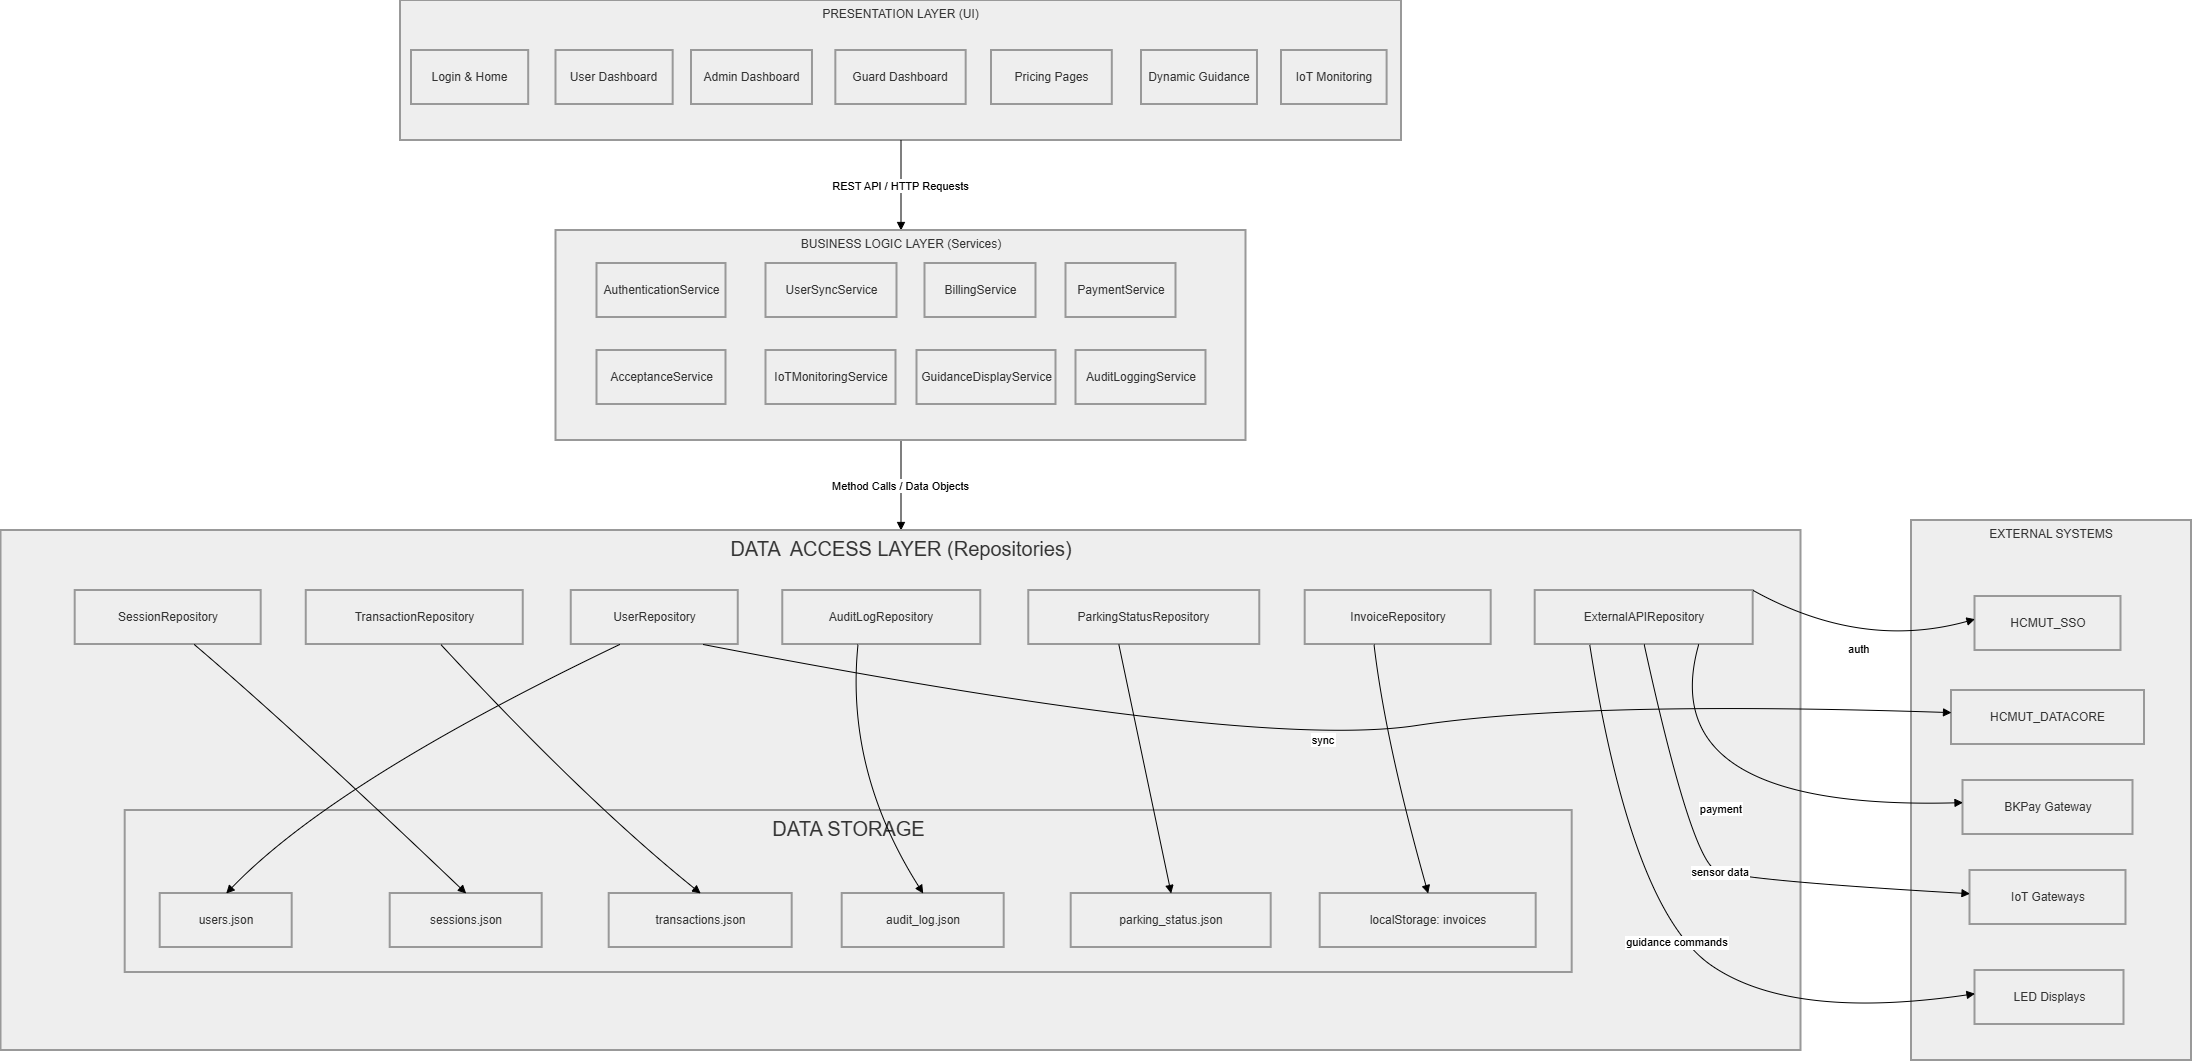
\includegraphics[width=1.0\textwidth]{pictures/implement_diagram/architecture_diagram.png}
    \caption{UML Component Diagram - Kiến trúc hệ thống IoT-SPMS}
    \label{arch_diagram}
\end{figure}

Sơ đồ trên thể hiện các thành phần chính (Components) và mối quan hệ giữa chúng:

\begin{itemize}
    \item \textbf{Web Interface}: Tất cả các giao diện người dùng (Admin, User, Guard, Pricing)
    
    \item \textbf{Service Layer}: Các dịch vụ xử lý logic nghiệp vụ (Authentication, BillingService, PaymentService, IoTMonitoring, GuidanceDisplay)
    
    \item \textbf{Repository Layer}: Các Repository để truy cập dữ liệu (User, Session, Transaction, Invoice, AuditLog)
    
    \item \textbf{External Systems}:
    \begin{itemize}
        \item HCMUT\_SSO: Xác thực
        \item HCMUT\_DATACORE: Đồng bộ dữ liệu
        \item BKPay: Thanh toán
        \item IoT Gateways: Cảm biến
    \end{itemize}
    
    \item \textbf{Data Storage}: Các tệp JSON lưu trữ dữ liệu nội bộ
\end{itemize}

\subsection{Sơ đồ triển khai}

\begin{figure}[H]
    \centering
    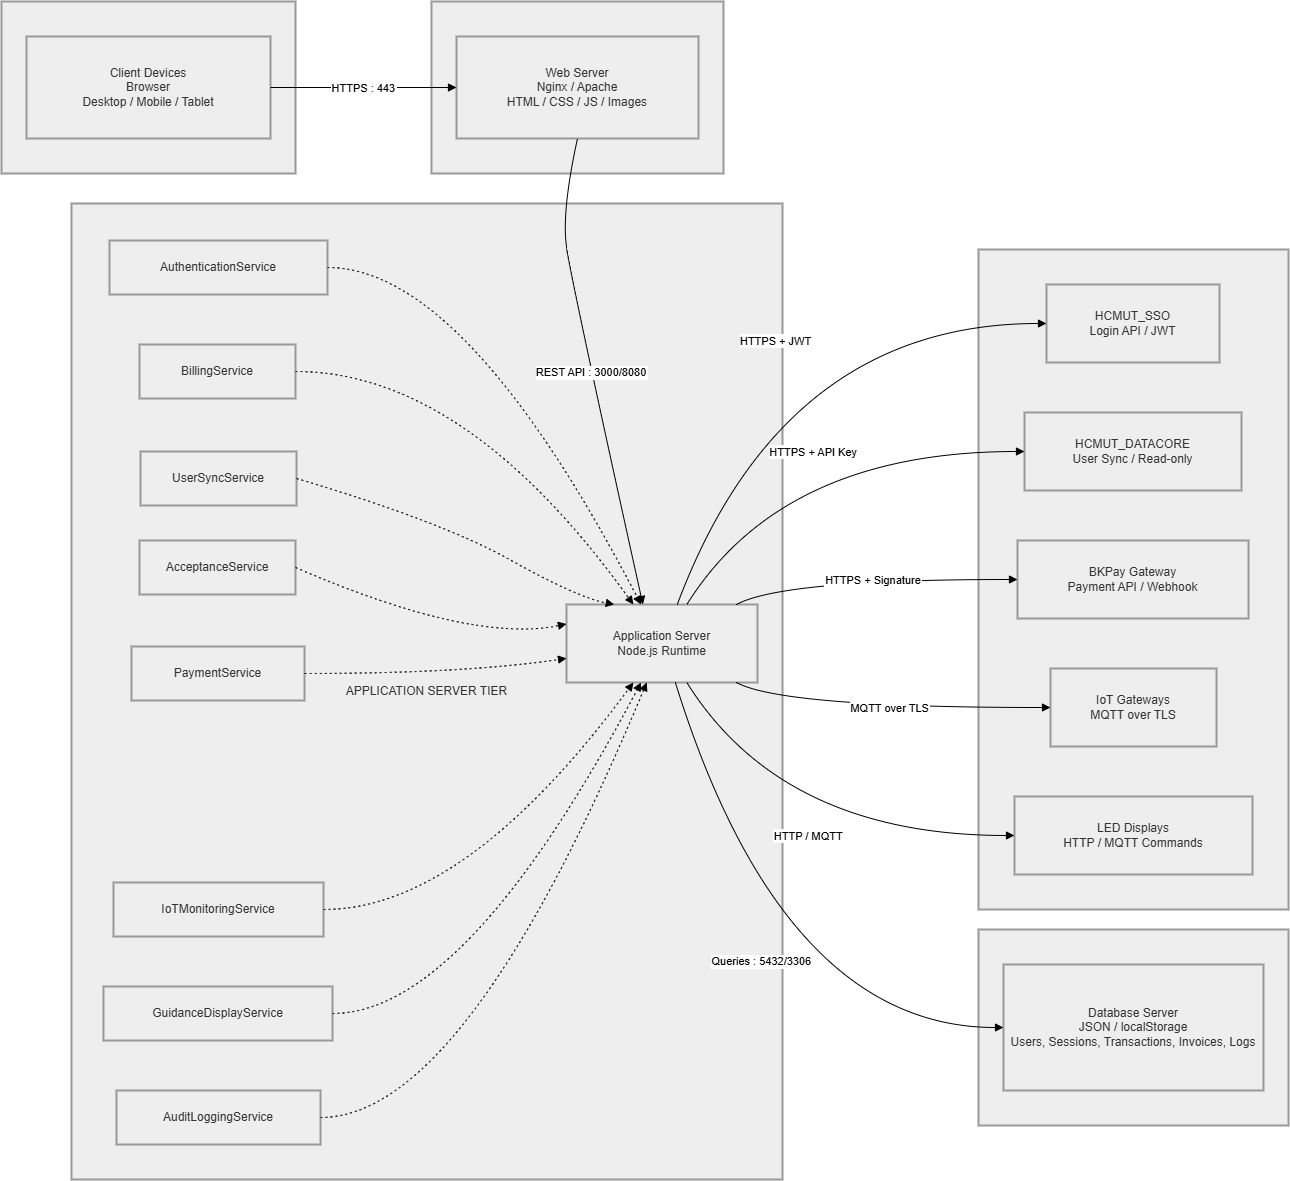
\includegraphics[width=1.0\textwidth]{pictures/implement_diagram/deployment_diagram.png}
    \caption{Deployment Diagram - Triển khai hệ thống IoT-SPMS}
    \label{deployment_diagram}
\end{figure}

Hệ thống được triển khai trên các nút (nodes) như sau:

\begin{itemize}
    \item \textbf{Client Devices}: Các máy tính, điện thoại di động của người dùng, được truy cập thông qua trình duyệt web (Browser)
    
    \item \textbf{Web Server}: Máy chủ web tĩnh (Static Web Server) chứa các tệp HTML, CSS, JavaScript và các tài nguyên web tĩnh. Có thể sử dụng Nginx, Apache hoặc Node.js Express.
    
    \item \textbf{Application Server}: Máy chủ ứng dụng chạy các dịch vụ business logic (NodeJS runtime với các Service modules). Thực hiện xử lý API requests, tính toán, xác thực.
    
    \item \textbf{Database Server}: Máy chủ lưu trữ dữ liệu:
    \begin{itemize}
        \item File-based JSON (users.json, sessions.json, transactions.json, audit\_log.json) cho development/testing
        \item Có thể mở rộng sang SQL Database (PostgreSQL, MySQL) cho production
    \end{itemize}
    
    \item \textbf{External Integration Nodes}:
    \begin{itemize}
        \item SSO Server: HCMUT\_SSO
        \item Data Server: HCMUT\_DATACORE
        \item Payment Gateway: BKPay
        \item IoT Gateway: Thiết bị gateway nhận dữ liệu từ các cảm biến bãi đỗ
        \item LED Display Controllers: Thiết bị điều khiển bảng LED
    \end{itemize}
    
    \item \textbf{Communication Protocols}:
    \begin{itemize}
        \item HTTPS: Kết nối web client - web server
        \item RESTful API: Kết nối web app - application server
        \item MQTT over TLS / HTTPS: Kết nối IoT devices - application server
        \item JWT / Session Tokens: Xác thực người dùng
    \end{itemize}
\end{itemize}

\subsection{Luồng triển khai (Luồng tương tác)}

\subsubsection{Luồng 1: Đăng nhập \& Phân quyền}

\begin{enumerate}
    \item Người dùng truy cập trang chủ (index.html), kích hoạt nút "Đăng nhập"
    \item Hệ thống điều hướng sang login.html
    \item Người dùng nhập thông tin tài khoản, hệ thống gửi yêu cầu xác thực tới HCMUT\_SSO
    \item HCMUT\_SSO trả về JWT token
    \item Hệ thống giải mã token, lấy thông tin role từ UserRepository
    \item Dựa trên role, người dùng được điều hướng:
    \begin{itemize}
        \item Role = 'admin' → admin/admin\_dashboard.html
        \item Role = 'guard' → guard/dashboard.html
        \item Role = 'user' → user/dashboard.html
    \end{itemize}
    \item AuditLoggingService ghi lại sự kiện login
\end{enumerate}

\subsubsection{Luồng 2: Đồng bộ dữ liệu người dùng}

\begin{enumerate}
    \item Quản trị viên truy cập admin/sync.html
    \item Nhấn nút "Khởi chạy đồng bộ"
    \item UserSyncService gọi API HCMUT\_DATACORE để lấy danh sách người dùng
    \item DATACORE trả về dữ liệu JSON
    \item UserSyncService lọc dữ liệu, thêm mới hoặc cập nhật vào users.json
    \item Ghi log thành công: "Synced X users"
    \item Cập nhật UI thể hiện kết quả
\end{enumerate}

\subsubsection{Luồng 3: Tính phí \& Tạo hóa đơn (Billing)}

\begin{enumerate}
    \item IoTMonitoringService ghi nhận Session (người dùng vào/ra bãi đỗ)
    \item Khi Session kết thúc (exit event), BillingService được gọi
    \item BillingService tính phí dựa trên:
    \begin{itemize}
        \item Duration = exit\_time - entry\_time
        \item User type từ UserRepository
        \item Pricing rules từ pricing\_config (được quản trị viên cấu hình)
    \end{itemize}
    \item BillingService tạo Invoice object (status = PENDING), gọi InvoiceRepository.upsertInvoice()
    \item Invoice được lưu vào localStorage (spms\_invoices\_v1)
    \item AuditLoggingService ghi: "Invoice created: INV-XXX, Amount: YYY VND"
\end{enumerate}

\subsubsection{Luồng 4: Thanh toán qua BKPay}

\begin{enumerate}
    \item Người dùng truy cập user/billing.html, xem danh sách Invoice (PENDING)
    \item Nhấn "Thanh toán ngay" trên một Invoice
    \item PaymentService.requestPayment(invoiceId) được gọi
    \item PaymentService cập nhật trạng thái Invoice: PENDING → PROCESSING
    \item PaymentService tạo Transaction object, gọi ExternalAPIRepository.initiateBKPayTransaction()
    \item BKPay Gateway trả về redirect URL
    \item Người dùng được điều hướng tới trang thanh toán BKPay
    \item Sau khi hoàn tất thanh toán, BKPay gửi callback về webhook endpoint
    \item PaymentService.processPaymentCallback() được gọi
    \item Kiểm tra idempotency (đã xử lý trước chưa?)
    \item Nếu SUCCESS: cập nhật Invoice status → SUCCESS, gọi DATACORE sync
    \item Nếu FAILED: cập nhật Invoice status → FAILED, ghi log lỗi
    \item AuditLoggingService ghi lại kết quả thanh toán
\end{enumerate}

\subsubsection{Luồng 5: Giám sát IoT \& Cập nhật trạng thái bãi đỗ}

\begin{enumerate}
    \item IoT Gateways gửi dữ liệu trạng thái (spot occupied/vacant) tới Application Server qua MQTT over TLS
    \item IoTMonitoringService nhận dữ liệu, cập nhật ParkingStatusRepository
    \item GuidanceDisplayService tính toán trạng thái tổng thể (vacant spots, occupancy rate)
    \item GuidanceDisplayService gửi lệnh điều khiển sang LED Display Controllers
    \item LED displays cập nhật thông tin trạng thái bãi đỗ (VD: "Còn 150 chỗ" → "Còn 149 chỗ")
    \item Cập nhật cũng được hiển thị trên web dashboard (admin/iot\_monitoring.html, guard/status.html)
    \item AuditLoggingService ghi các sự kiện quan trọng (device offline, sensor error, v.v.)
\end{enumerate}

\subsubsection{Luồng 6: Điều hướng giao thông (Dynamic Guidance)}

\begin{enumerate}
    \item GuidanceDisplayService tính toán mức độ tiêu hao bãi: vacant\% = remainingSpots / totalSpots × 100
    \item Dựa trên ngưỡng cấu hình:
    \begin{itemize}
        \item Còn > 30\% chỗ → Trạng thái "GreenLight" (Xanh), hiển thị "Còn chỗ"
        \item 10\% < chỗ ≤ 30\% → Trạng thái "YellowLight" (Vàng), hiển thị "Gần đầy"
        \item Chỗ ≤ 10\% → Trạng thái "RedLight" (Đỏ), hiển thị "Hết chỗ"
    \end{itemize}
    \item GuidanceDisplayService gửi lệnh API tới LED Display Controllers
    \item Các bảng LED hiển thị tính từ các điểm đầu vào chính (entry gates)
    \item Quản trị viên có thể quản lý nội dung hiển thị qua dynamic\_guidance/admin-control.html
\end{enumerate}

\subsubsection{Luồng 7: Ghi nhật ký kiểm toán (Audit Logging)}

\begin{enumerate}
    \item Mỗi sự kiện quan trọng (login, sync, payment, invoice update, etc.) được ghi lại bởi AuditLoggingService
    \item Mỗi audit log entry chứa:
    \begin{itemize}
        \item \texttt{timestamp}: Thời gian xảy ra sự kiện (ISO format)
        \item \texttt{severity}: Mức độ (INFO, WARNING, ERROR, CRITICAL)
        \item \texttt{actor}: Ai thực hiện (user id, system, admin name)
        \item \texttt{action}: Hành động gì (login, sync, payment, etc.)
        \item \texttt{status}: Kết quả (Success, Failed, Pending)
        \item \texttt{details}: Chi tiết bổ sung
        \item \texttt{metadata}: Thông tin tham chiếu (invoice id, user id, etc.)
    \end{itemize}
    \item Audit logs được lưu vào audit\_log.json và hiển thị trên admin/logs.html
    \item Quản trị viên có thể xuất báo cáo, lọc theo khoảng thời gian, actor, severity
\end{enumerate}

\subsection{Tóm tắt công nghệ}

Hệ thống IoT-SPMS sử dụng stack công nghệ sau:

\begin{table}[H]
    \centering
    \begin{tabularx}{\textwidth}{|l|X|l|}
    \hline
    \textbf{Tầng} & \textbf{Thành phần} & \textbf{Công nghệ} \\
    \hline
    \multirow{4}{*}{\textbf{Presentation}} 
    & Markup & HTML5 \\
    & Styling & CSS3 + Design System (Dark Mode) \\
    & Scripting & JavaScript (Vanilla / ES6+) \\
    & Framework UI & Không sử dụng (Pure web) \\
    \hline
    \multirow{5}{*}{\textbf{Business Logic}} 
    & Runtime & Node.js \\
    & Service Implementation & JavaScript / ES6+ \\
    & Authentication & JWT + HCMUT\_SSO \\
    & Payment Processing & BKPay API Integration \\
    & IoT Communication & MQTT over TLS / HTTPS \\
    \hline
    \multirow{4}{*}{\textbf{Data Access}} 
    & Local Storage & JSON files \\
    & Session Storage & Browser sessionStorage \\
    & Caching & Browser localStorage \\
    & External APIs & REST API \\
    \hline
    \multirow{2}{*}{\textbf{Infrastructure}} 
    & Web Server & Nginx / Apache / Node.js Express \\
    & Deployment & Docker (optional) \\
    \hline
    \multirow{3}{*}{\textbf{DevOps}} 
    & Version Control & Git \\
    & Build Tools & LaTeX (cho tài liệu) \\
    & Documentation & Markdown + LaTeX \\
    \hline
    \end{tabularx}
    \caption{Technology Stack của hệ thống IoT-SPMS}
    \label{tech_stack}
\end{table}

\subsection{Chi tiết triển khai chính}

\subsubsection{Quản lý trạng thái thanh toán}

Hệ thống quản lý trạng thái hóa đơn (Invoice) theo mô hình State Machine:

\begin{table}[H]
    \centering
    \begin{tabularx}{\textwidth}{|l|X|l|}
    \hline
    \textbf{Trạng thái} & \textbf{Ý nghĩa} & \textbf{Chuyển đổi sang} \\
    \hline
    PENDING & Hóa đơn đã tạo, chưa thanh toán & PROCESSING, CANCELLED \\
    PROCESSING & Đang chờ kết quả từ BKPay & SUCCESS, FAILED, CANCELLED \\
    SUCCESS & Thanh toán thành công & (kết thúc) \\
    FAILED & Thanh toán thất bại & PROCESSING (retry), CANCELLED \\
    CANCELLED & Hóa đơn bị hủy & PROCESSING (pay again) \\
    \hline
    \end{tabularx}
    \caption{Invoice State Machine Transitions}
    \label{invoice_state}
\end{table}

\subsubsection{Cơ chế idempotency cho webhook}

PaymentService triển khai cơ chế idempotency cho webhook callback từ BKPay bằng cách lưu trữ Transaction status. Khi nhận callback lặp cùng transaction ID, hệ thống sẽ:
\begin{itemize}
    \item Kiểm tra xem transaction đã được xử lý chưa
    \item Nếu đã xử lý (status ≠ PENDING), bỏ qua callback
    \item Nếu chưa, tiến hành xử lý và cập nhật status
\end{itemize}

Điều này đảm bảo:
\begin{itemize}
    \item Không thanh toán trùng
    \item Trạng thái luôn nhất quán
    \item Audit log rõ ràng
\end{itemize}

\subsubsection{Chiến lược đồng bộ hóa dữ liệu}

\begin{itemize}
    \item \textbf{User Data}: Đồng bộ định kỳ từ DATACORE (caching locally)
    \item \textbf{Session Data}: Được cập nhật real-time khi IoT events xảy ra
    \item \textbf{Transaction Data}: Lưu immediately khi khởi tạo, cập nhật khi nhận callback
    \item \textbf{Parking Status}: Updated real-time từ IoT Gateways (near real-time, max 5 sec delay)
\end{itemize}

\subsubsection{Chiến lược xử lý lỗi}

Hệ thống triển khai chiến lược xử lý lỗi toàn diện:

\begin{itemize}
    \item \textbf{Connection Loss}: Hệ thống sử dụng dữ liệu cache lưu trữ cuối cùng
    \item \textbf{Timeout}: Thiết lập timeout rõ ràng (8 giây cho BKPay, 8 giây cho DATACORE)
    \item \textbf{Payment Failure}: Cho phép retry, ghi log chi tiết mã lỗi
    \item \textbf{IoT Device Offline}: Ghi cảnh báo, tiếp tục hoạt động với dữ liệu lưu trữ
    \item \textbf{Database Error}: Rollback transaction nếu thất bại ở giữa quá trình
\end{itemize}

\subsection{Cân nhắc về bảo mật}

\begin{itemize}
    \item \textbf{Authentication}: Sử dụng JWT + HCMUT\_SSO, không lưu password
    \item \textbf{Authorization}: RBAC (Role-Based Access Control) với 4 vai trò: user, guard, admin, system
    \item \textbf{Data Protection}: HTTPS cho tất cả kết nối; MQTT over TLS cho IoT
    \item \textbf{Payment Security}: HMAC signature cho BKPay requests; không lưu trữ thông tin ngân hàng
    \item \textbf{Audit Trail}: Mọi hành động được ghi log để truy vết
    \item \textbf{Input Validation}: Kiểm tra và sanitize toàn bộ user input
\end{itemize}

\subsection{Tổng kết}

Implementation View của hệ thống IoT-SPMS được thiết kế theo kiến trúc phân tầng chuẩn với 3 tầng chính (Presentation, Business Logic, Data Access). Hệ thống tích hợp seamlessly với các hệ thống bên ngoài (SSO, DATACORE, BKPay, IoT Gateways) thông qua các API endpoint và protocols chuẩn. Mỗi thành phần được triển khai với các hành động cụ thể (interaction flows) đảm bảo tính chính xác, an toàn, và khả năng chịu lỗi. Technology stack được lựa chọn đơn giản nhưng hiệu quả: HTML5/CSS3/JavaScript cho frontend, Node.js cho backend, JSON để lưu trữ, và các API chuẩn để tích hợp. Chiến lược xử lý lỗi, đồng bộ dữ liệu, và quản lý trạng thái được triển khai toàn diện để đảm bảo hệ thống hoạt động ổn định 24/7 trong môi trường sản xuất.
